\section{Model Selection}

Model selection is handled in three stages. First, the xLSTM sweep identifies the strongest configuration among the tokenizer, batch-size, scale, and schedule variants. Second, that derived xLSTM setup is used to define matched Transformer baselines rather than treating GPT-2 and LLaMA as independent, separately tuned systems. Third, the selected xLSTM, GPT-2-style, and LLaMA-style checkpoints are compared with the same held-out generation procedure.

During xLSTM training, the trainer selects checkpoints by validation loss. Whenever an evaluation step improves the run's validation loss, the checkpoint is copied to the run-local \verb|best/checkpoint.pt| path. This gives every xLSTM run a reproducible first-stage checkpoint tied to the same next-token objective used for optimization.

Across xLSTM runs, the first-stage comparison uses the exported \verb|summary.json| files and W\&B histories rather than the final checkpoint alone. This distinction matters because several runs overfit or degrade after their best validation step. The clearest example is the 15-epoch medium tokenizer-14 run: its best validation loss is 1.5173 at step 9000, but the final validation loss is 1.8799 after 72,870 steps. The selected checkpoint for that run is therefore the early best checkpoint, not the final training state.

\begin{table}[htbp]
	\centering
	\scriptsize
	\begin{tabular}{lrrrrr}
		\toprule
		Run                                                 & Params & Tok. & Batch & Best val. loss  \\
		\midrule
		\texttt{tok\_14\_batch\_16}                         & 3.70M  & 14   & 16    & \textbf{1.4456} \\
		\texttt{tok\_14} / \texttt{tok\_14\_batch\_8}       & 3.70M  & 14   & 8     & 1.4471          \\
		\texttt{tok\_10\_batch\_4}                          & 3.67M  & 10   & 4     & 1.4575          \\
		\texttt{tok\_10} / \texttt{tok\_10\_batch\_8}       & 3.67M  & 10   & 8     & 1.4619          \\
		\texttt{tok\_10\_batch\_16}                         & 3.67M  & 10   & 16    & 1.4663          \\
		\texttt{tok\_10\_chords}                            & 3.68M  & 10   & 8     & 1.4690          \\
		\texttt{tok\_14\_chords}                            & 3.70M  & 14   & 8     & 1.4823          \\
		\texttt{xlstm-medium-batch8-tok14-15epoch-restarts} & 9.28M  & 14   & 8     & 1.5173          \\
		\bottomrule
	\end{tabular}
	\caption{Current first-stage model candidates ranked by best validation loss. The ranking uses validation summaries only and should be revisited after held-out generation evaluation.}
	\label{tab:model-selection-candidates}
\end{table}

The current first-stage xLSTM candidate is the base xLSTM with tokenizer 14. The best scalar validation loss is the batch-16 run, but the batch-8 tokenizer-14 run is effectively tied and is the safer practical default for subsequent experiments because it leaves more memory headroom for larger models and generation-time diagnostics. The tokenizer-10 runs are close enough to remain useful baselines, while tokenizer 11 is no longer the preferred downstream representation despite being the tokenizer-only autotune winner.

\begin{figure}[htbp]
	\centering
	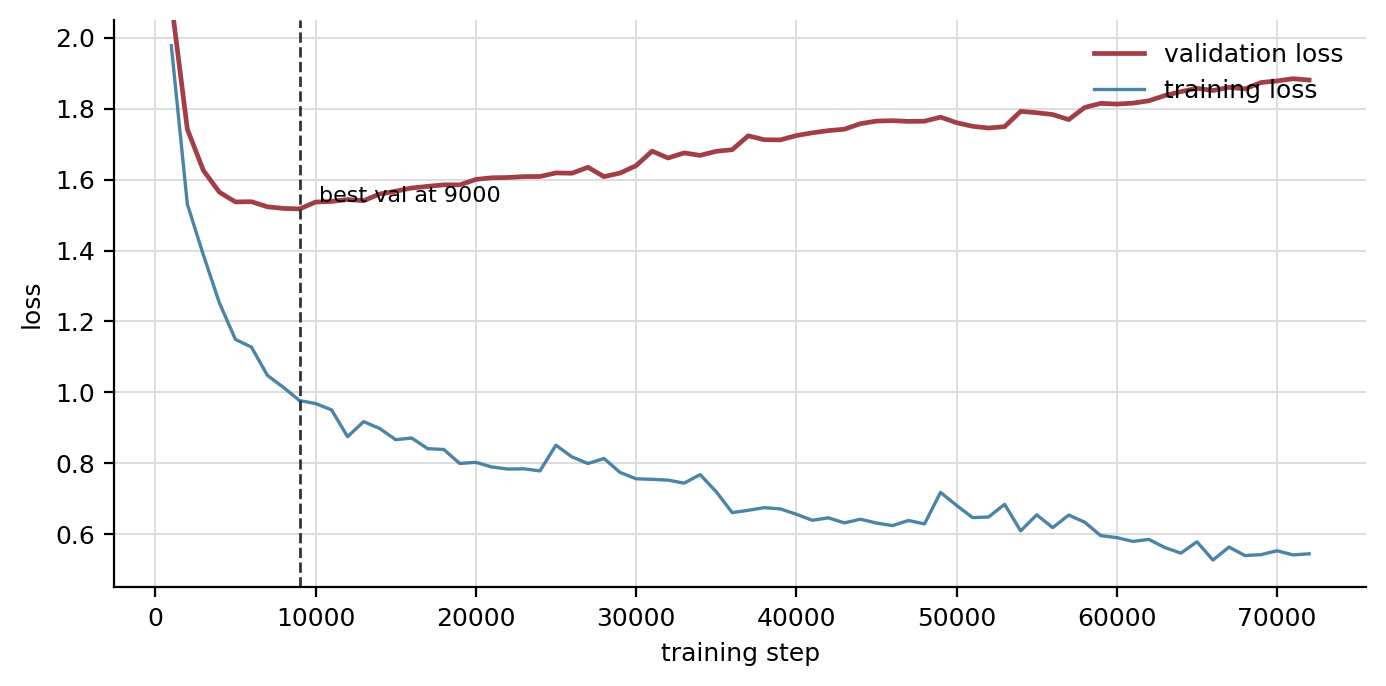
\includegraphics[width=0.90\textwidth]{figures/xlstm_medium_overfit_curve.png}
	\caption{Training and validation loss for the medium tokenizer-14 run. The widening gap after step 9000 shows why final-checkpoint selection would be misleading for this experiment.}
	\label{fig:xlstm-medium-overfit}
\end{figure}

The medium run is therefore useful as a negative selection example. It was derived from sensible sweep conclusions--tokenizer 14, batch size 8, and a larger model--but its W\&B trajectory indicates that more capacity and longer training did not translate into a better validation checkpoint under the chosen schedule. The correct action is not to select the final medium checkpoint, nor to treat the medium architecture as ruled out. The correct action is to keep the early best checkpoint as an evaluated candidate and require a follow-up medium sweep before claiming that the larger model improves generation quality.

The Transformer baselines are introduced after this xLSTM selection step. The launcher \path{experiments/run_transformer_tok14_gpt2_llama.sh} trains the GPT-2-style and LLaMA-style models sequentially with the same split files, tokenizer 14, block size 1024, and comparison training configuration. The two model YAML files, \path{configs/model/transformer/tok_14_gpt2_match.yaml} and \path{configs/model/transformer/tok_14_llama_match.yaml}, keep the Transformer models close to the selected xLSTM scale while changing the sequence-modeling architecture. This makes the Transformer runs controlled baselines for the xLSTM-derived setup instead of a separate hyperparameter search.

The Transformer training pipeline uses \path{scripts/train_gpt2.sh} for both architectures. Despite the wrapper name, the selected model YAML decides whether \verb|src.models.Transformer.train| instantiates the GPT-2-style or LLaMA-style configuration. The shared training YAML, \path{configs/train/transformer_tok14_batch16_sched_decay8000.yaml}, fixes the batch size, epoch budget, validation interval, checkpoint interval, W\&B project, and block size used by both Transformer baselines. Checkpoint selection follows the Hugging Face training path described earlier: validation loss is the selection metric, the best validation checkpoint is loaded at the end of training, and the selected model is saved in the run directory for later generation and scoring.

This means that the comparison set contains three selected training artifacts: the best xLSTM checkpoint from the tokenizer-14 xLSTM sweep, the GPT-2-style Transformer trained from the matched tokenizer-14 configuration, and the LLaMA-style Transformer trained from the same matched comparison recipe. The Transformer models are not chosen because they won the xLSTM sweep; they are included because they test whether a decoder-only Transformer architecture performs differently when trained under the same symbolic-music representation and comparable training conditions.

Validation loss is still only a proxy for musical quality. It measures the probability assigned to the next reference token, not whether sampled continuations decode cleanly or have musical statistics close to the held-out references. For final selection, the validation-ranked checkpoints and the matched Transformer baselines should therefore be evaluated with the generation and scoring pipeline already described in the training setup. The repository first generates MIDI continuations from held-out prompts and records decode success. The scoring stage then computes MusPy descriptors \citep{dongMusPyToolkitSymbolic2020} for each generated MIDI and its reference, stores descriptor-level absolute differences, and aggregates a Frechet Music Distance score \citep{retkowskiFrechetMusicDistance2025} over the generated and reference MIDI sets.

The final model choice should use a two-gate rule. A checkpoint first has to be competitive on validation loss and perplexity, because a model with poor next-token behavior is unlikely to be a strong generator. Among the validation-competitive checkpoints, the selected model should then be the one with the strongest held-out generation behavior: high decode and score success, small MusPy differences from the reference set \citep{dongMusPyToolkitSymbolic2020}, low Frechet Music Distance \citep{retkowskiFrechetMusicDistance2025}, and acceptable qualitative MIDI inspection. Under that rule, the xLSTM validation ranking identifies the recurrent checkpoint that should enter the comparison, and the matched Transformer pipeline defines the GPT-2-style and LLaMA-style counterparts that should be evaluated against it.
